
\documentclass[a4paper,14pt]{extarticle}
\usepackage[utf8]{inputenc}
\usepackage[english,russian]{babel}

\usepackage{tikz}

\usepackage{setspace}
\singlespacing % одинарный интервал

\usepackage{amsmath}
\usepackage{amsfonts}
\usepackage{amssymb}
\usepackage{mathtext}
\usepackage{graphicx}
\usepackage{float}
\usepackage[left=3cm, right=1cm, top=1.5cm, bottom=1.5cm]{geometry}
\usepackage{icomma} % "Умная" запятая: $0,2$ --- число, $0, 2$ --- перечисление
\usepackage{indentfirst} % Красная строка.

\usepackage{minted}

\renewcommand{\thesection}{\arabic{section}}

\begin{document}
\begin{titlepage}
  \begin{center}
    ГОУ ВО АЛТАЙСКИЙ ГОСУДАРСТВЕННЫЙ УНИВЕРСИТЕТ
    \vspace{0.25cm}
    
    Физико-технический факультет
    
    Кафедра вычислительной техники и электроники
    \vfill
    
    {\LARGE Сеть в ОС GNU/Linux, MS Windows}\\[5mm]
    \textsc{(Отчёт по индивидуальному заданию по курсу <<Операционные системы>>)}
  \bigskip

\end{center}
\vfill

\newlength{\ML}
\settowidth{\ML}{«\underline{\hspace{0.7cm}}» \underline{\hspace{2cm}}}
\hfill\begin{minipage}{0.4\textwidth}
  Выполнил студент 2-го курса, 585 группы:\\
  \underline{\hspace{\ML}} А.\,К.~Роженцев\\
  «\underline{\hspace{0.7cm}}» \underline{\hspace{2cm}} \the\year~г.
\end{minipage}%
\bigskip

\hfill\begin{minipage}{0.4\textwidth}
  Проверил\\
  \underline{\hspace{\ML}} П.\,Н.~Уланов\\
  «\underline{\hspace{0.7cm}}» \underline{\hspace{2cm}} \the\year~г.
\end{minipage}%
\vfill

\begin{center}
  Барнаул, \the\year~г.
\end{center}
\end{titlepage}

%\maketitle

\tableofcontents
\newpage
\section{Сеть и виды сетей} %Сеть в ОС GNU/Linux, MS Windows


\centering

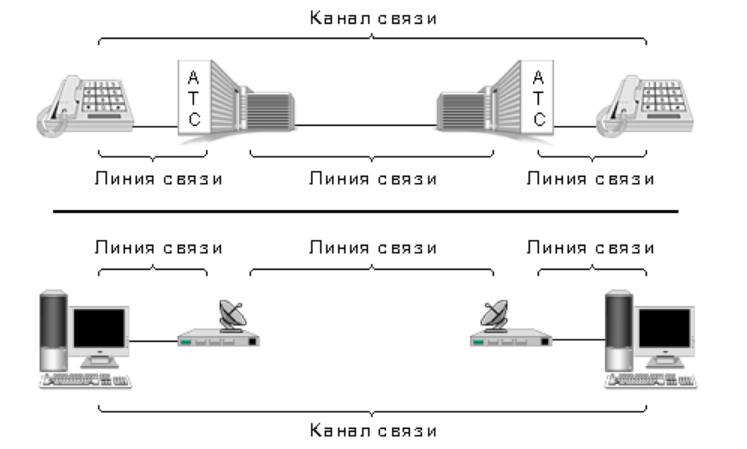
\includegraphics[width=0.8\linewidth]{n1.png}
\newline
\caption{Линии и канал связи}\\

Компьютерная сеть (Computer Network) – это множество компьютеров, соединенных линиями связи и работающих под управлением специального программного обеспечения.

Под линией связи обычно понимают совокупность технических устройств, и физической среды, обеспечивающих передачу сигналов от передатчика к приемнику. В реальной жизни примерами линий связи могут служить участки кабеля и усилители, обеспечивающие передачу сигналов между коммутаторами телефонной сети. На основе линий связи строятся каналы связи.

Каналом связи обычно называют систему технических устройств и линий связи, обеспечивающую передачу информации между абонентами. Соотношение между понятиями "канал" и "линия" описывается следующим образом: канал связи может включать в себя несколько разнородных линий связи, а одна линия связи может использоваться несколькими каналами







\centering
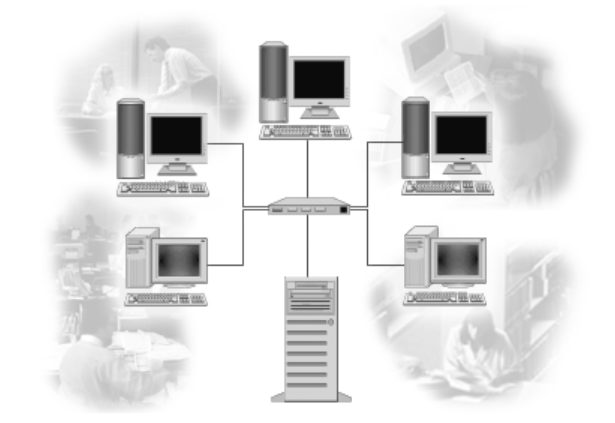
\includegraphics[width=0.75\linewidth]{n2.png}
\newline
\caption{Локальные сети(LAN)}\\
К локальным сетям (Local Area Network, LAN) обычно относят сети, компьютеры которых сосредоточены на относительно небольших территориях (как правило, в радиусе до 1-2 км). Классическим примером локальных сетей является сеть одного предприятия, расположенного в одном или нескольких стоящих рядом зданиях. Небольшой размер локальных сетей позволяет использовать для их построения достаточно дорогие и высококачественные технологии, что обеспечивает высокую скорость обмена информацией между компьютерами.





\centering
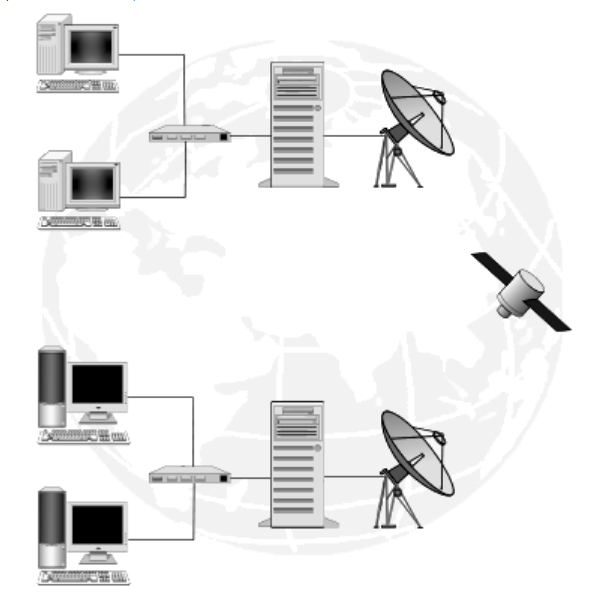
\includegraphics[width=0.9\linewidth]{n3.png}
\newline
\caption{Глобальные сети}\\
Глобальные сети (Wide Area Network, WAN) – это сети, предназначенные для объединения отдельных компьютеров и локальных сетей, расположенных на значительном удалении (сотни и тысячи километров) друг от друга. Поскольку организация специализированных высококачественных каналов связи большой протяженности является достаточно дорогой, то в глобальных сетях нередко используются уже существующие и изначально не предназначенные для построения компьютерных сетей линии (например, телефонные или телеграфные). В связи с этим скорость передачи данных в таких сетях существенно ниже, чем в локальных.






\centering
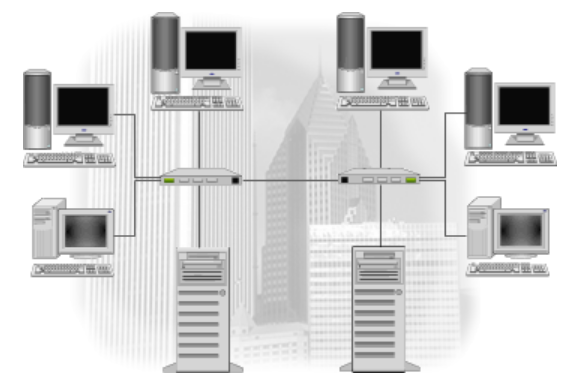
\includegraphics[width=0.9\linewidth]{n4.png}
\newline
\caption{Городские сети}\\
Не так давно к двум указанным типам сетей добавился еще один – так называемые городские сети (Metropolitan Area Network, MAN). Такие сети предназначены для обеспечения взаимодействия компьютеров и/или локальных сетей, рассредоточенных на территории крупного города (как правило, в радиусе до 100 км), а также для подключения локальных сетей к глобальным. Для построения таких сетей используются достаточно качественные цифровые линии связи, позволяющие осуществлять взаимодействие на относительно высоких по сравнению с глобальными сетями скоростях.


\centering
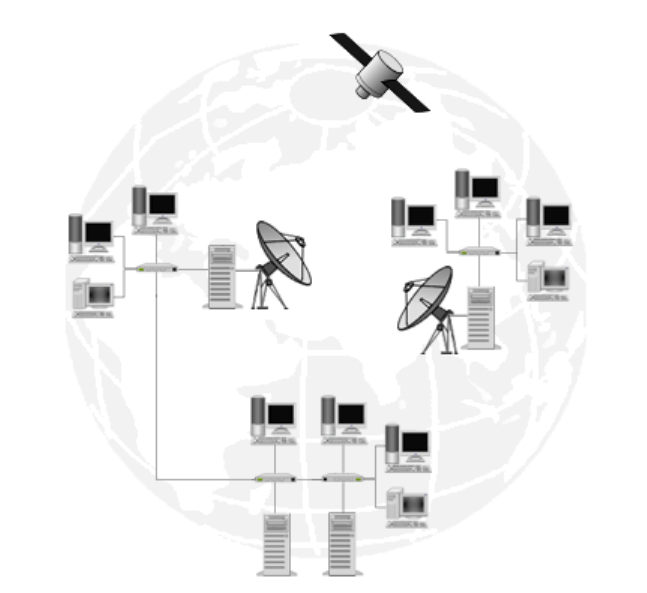
\includegraphics[width=0.9\linewidth]{n5.png}
\newline
\caption{Интернет}\\
Независимо от того, какую территорию покрывает сеть, какие технологические решения лежат в основе ее организации, существуют общие принципы сетевого взаимодействия, которым должно подчиняться функционирование сети. Именно выработка таких общих принципов способствовала в свое время появлению Интернет (Internet) как объединенной сети (иногда даже используется термин "гиперсеть"), собравшей в своем составе локальные, городские и глобальные сети всей планеты.


\newpage
\section{Домен,IP-адрес,Интернет}




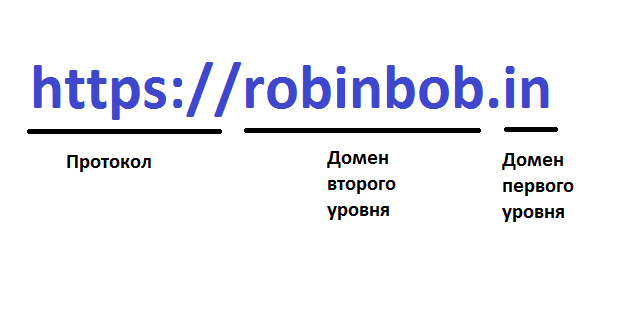
\includegraphics[width=1\linewidth]{domen.png}

Доме́нное имя — символьное имя, служащее для идентификации областей, которые являются единицами административной автономии в сети Интернет, в составе вышестоящей по иерархии такой области. Каждая из таких областей называется доме́ном.
\label{fig:mpr}
\newpage




\centering
IP-адрес — уникальный сетевой адрес узла в компьютерной сети, построенной на основе стека протоколов TCP/IP. В сети Интернет требуется глобальная уникальность адреса; в случае работы в локальной сети требуется уникальность адреса в пределах сети.
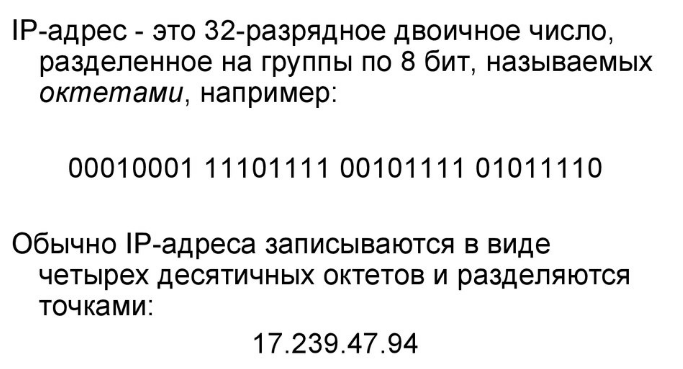
\includegraphics[width=1\linewidth]{ip.png}
\label{fig:mpr}
\newpage





\includegraphics[width=1\linewidth]{net.jpg}
Интерент - всемирная информационная компьютерная сеть, связывающая между собой как пользователей компьютерных сетей, так и пользователей индивидуальных компьютеров для обмена информацией.
\label{fig:mpr}


\section{Пакет(сетевые технологии)}
В компьютерных сетях пакет — это определённым образом оформленный блок данных, передаваемый по сети в пакетном режиме. Компьютерные линии связи, которые не поддерживают пакетного режима, как, например, традиционная телекоммуникационная связь точка-точка, передают данные просто в виде последовательности байтов, символов или битов поодиночке. Если данные сформированы в пакеты, битрейт коммуникационной среды можно более эффективно распределить между пользователями, чем в сети с коммутацией каналов. При использовании сетей с коммутацией пакетов можно надёжно гарантировать пороговый битрейт, ниже которого он опускаться не будет.

\newpage

\section{Протокол,HTTP,HTTPS,FTP}
Протокол передачи данных — набор соглашений интерфейса логического уровня, которые определяют обмен данными между различными программами. Эти соглашения задают единообразный способ передачи сообщений и обработки ошибок.\newline

HTTP (англ. HyperText Transfer Protocol — «протокол передачи гипертекста») — протокол прикладного уровня передачи данных изначально — в виде гипертекстовых документов в формате «HTML», в настоящий момент используется для передачи произвольных данных.\newline
\newline
HTTPS (англ. HyperText Transfer Protocol Secure) — расширение протокола HTTP для поддержки шифрования в целях повышения безопасности. Данные в протоколе HTTPS передаются поверх криптографических протоколов TLS или устаревшего в 2015 году SSL. В отличие от HTTP с TCP-портом 80, для HTTPS по умолчанию используется TCP-порт 443.
Протокол был разработан компанией Netscape Communications для браузера Netscape Navigator в 1994 году.\newline

FTP — протокол передачи файлов по сети, является одним из старейших прикладных протоколов, появившихся задолго до HTTP, и даже до TCP/IP, в 1971 году; в первое время он работал поверх протокола NCP. Он и сегодня широко используется для распространения ПО и доступа к удалённым хостам.\newline

\section{Порт}

Порт — целое неотрицательное число, записываемое в заголовках протоколов транспортного уровня модели OSI. Используется для определения процесса-получателя пакета в пределах одного хоста.\newline

В заголовках протоколов TCP и UDP для хранения номеров портов выделены поля размером 16 бит. Для протокола TCP порт с номером 0 зарезервирован и не может использоваться. Для протокола UDP указание порта процесса-отправителя («обратного» порта) не является обязательным, и порт с номером 0 означает отсутствие порта. Таким образом, номер порта — число в диапазоне от 1 до 216-1=65 535.\newline

В системах GNU Linux существует утилита под название NMAP при помощи которой можно к примеру, просканировать порты.\newline

Команда: nmap IP-ADDRES 

\newpage

\section{Конец}



\end{document} 

